\documentclass[14pt]{beamer}
\usepackage{beamerthemesplit}
\usepackage{graphicx}
\usetheme{CambridgeUS}
\usefonttheme{serif}
\usepackage{bookman}
\usepackage{xcolor}

\title{SPIN}

\subtitle{Student Performance Information Network}

\author[Damini Charvitha Lendi]{K.Damini Satya \\ K.Sri Charvitha \\ M.Lendi Vihari }

\institute[BVRITH]{Department of Computer Science Engineering and Information Technology}

\begin{document}


\maketitle

\begin{frame}

\frametitle{Information Overload}

	\begin{columns}[T]

		\begin{column}{.55\textwidth}
		\vspace{8mm}
		\includegraphics[scale = 0.6]{crowd.jpeg}

				\begin{itemize}
					
					\item  What is happening? 

					\item How are we doing?

				\end{itemize}

		\end{column}

		\begin{column}{.45\textwidth}
		
		       \includegraphics[scale = 0.44]{learn.jpeg}
		       
			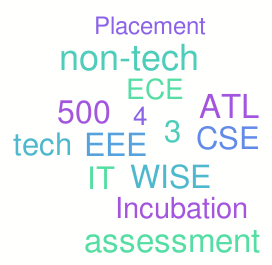
\includegraphics[scale = 0.38]{tag1.png}

		\end{column}

	\end{columns} 

\end{frame}


\begin{frame}

\frametitle{Silver Bullet}

SPIN - A common platform for students and management.

	\begin{center}

		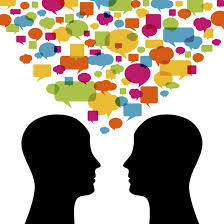
\includegraphics[scale = 0.4]{interact.jpeg}

	\end{center}

\end{frame}


\begin{frame}

\frametitle{Purpose}

\begin{block}{Student View}

	\begin{itemize}
	
	\item Get notified with tech and non-tech information.
	
	\item Aid to improve Personality.
	
	\end{itemize}

\end{block}

\begin{block}{Management Perspective}

	\begin{itemize}

		\item Analyse overall performance of students.

		\item Know details of the programs. 

		\item Know the effectiveness of the programs being conducted.

	\end{itemize}

\end{block}

\end{frame}


\begin{frame}{Application Taxonomy}

	\begin{center}

	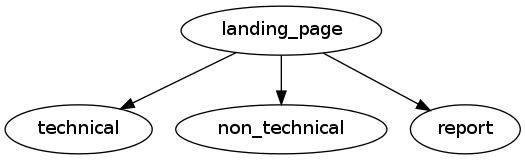
\includegraphics[scale = 0.45]{spin.png}

	\end{center}

\end{frame}


\begin{frame}{Application Taxonomy}

	\begin{center}

	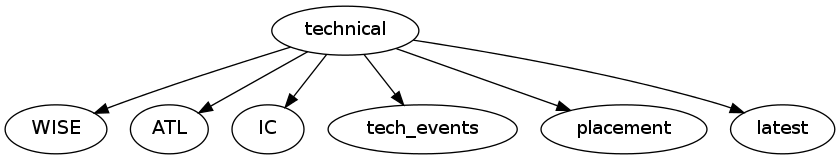
\includegraphics[scale = 0.38]{tech.png}

	\end{center}

\end{frame}


\begin{frame}{Application Taxonomy}

	\begin{center}

	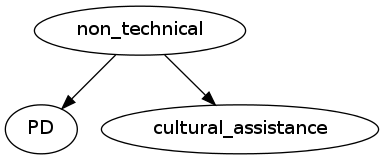
\includegraphics[scale = 0.5]{nontech.png}

	\end{center}

\end{frame}


\begin{frame}{Application Taxonomy}

	\begin{center}

	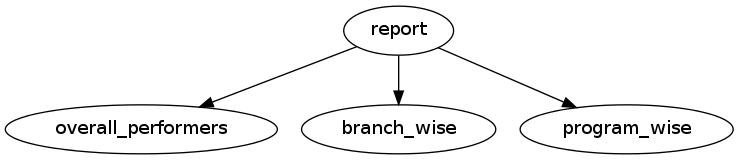
\includegraphics[scale = 0.4]{report.png}

	\end{center}

\end{frame}

\begin{frame}{Modules}

	\begin{block}{Notification Module}

		Notifications Delivered.

	\end{block}

	\begin{block}{Assessment Module}

		Student Achievements showcased.

	\end{block}

	\begin{block}{Admin Module}

		\begin{itemize}

		\item Publish the content to be notified.

		\item Maintain database.

		\end{itemize}

	\end{block}

\end{frame}


\begin{frame}{Learnt}

	\begin{itemize}

		\item Project Development Cycle

		\item Database Designing

		\item JDBC

		\item Servlets

		\item Inotify

		\item Graphviz

		\item Text Processing and Code Generation

	\end{itemize}

	\begin{center}

		\includegraphics[scale=0.35]{insert.png}

	\end{center}

\end{frame}


\begin{frame}{Tools}

	\begin{itemize}

		\item HTML,CSS,JQuery

		\item Eclipse IDE for Java EE Developers

		\item Apache tomcat 7

		\item MySQL

	\end{itemize}

\end{frame}


\begin{frame}{Coming Up}

	\begin{itemize}

		\item Discussion Forum

		\item User Posting
		
		\item Security

	\end{itemize}

	\begin{center}

		\includegraphics[scale=0.35]{FS.jpg}	

	\end{center}

\end{frame}



\begin{frame}

	\begin{center}

		
\includegraphics[scale=0.3]{ty.jpg}

	\end{center}

\end{frame}

\end{document}